\section{多级继承}
任何一个自定义类型都可以作为基类,被其它类继承,从而成为其它类的一部分\footnote{有一种例外:标注为 \lstinline@final@ 的类不可以被继承。但本书不打算讲解 \lstinline@final@ 的相关内容。}。对于公有继承来说,这相当于是对基类对象所拥有的共性,添加了一些派生类对象额外的特性;对于私有继承来说,这相当于是把一个基类的对象内嵌到派生类中,作为它的一个成员。\par
接下来我们还可以把派生类再作为基类,用它来继承新的类。我们把这种操作叫作\textbf{多级继承(Multilevel inheritance)}。
\begin{lstlisting}
struct A { /*...*/ };
struct B : A { /*...*/ }; //B继承自A
struct C : B { /*...*/ }; //C继承自B
class D : C { /*...*/ }; //D继承自C
\end{lstlisting}
看上去好像很复杂,但是读者只需要把握刚才那点就可以理顺各种关系。对于这个继承关系来说,\lstinline@B@ 继承了 \lstinline@A@ 的共性又有自己的特性;\lstinline@C@ 继承了 \lstinline@B@ 的共性并有了自己的特性;\lstinline@D@ 稍有不同,它私有继承自 \lstinline@C@,表示的是 \lstinline@D@ 中内嵌了一个 \lstinline@C@ 对象作为其成员。\par
当然,这是一个虚构的例子,不那么形象。现在我们就来看两个真实的例子。\par
\subsection*{生物分类法}
\begin{figure}[htbp]
    \centering
    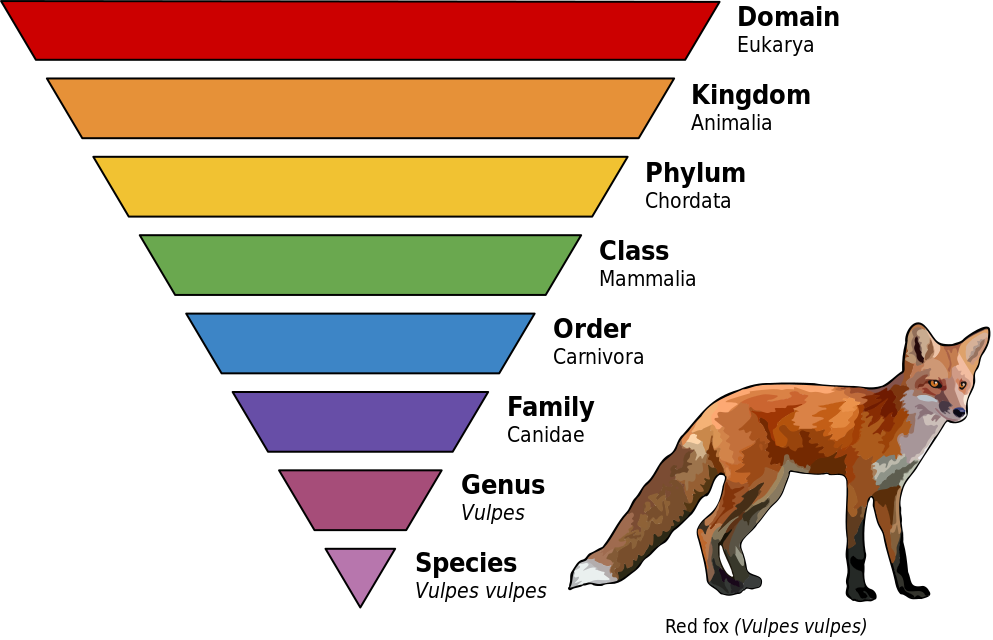
\includegraphics[width=.75\textwidth]{../images/generalized_parts/09_taxonomic_rank_graph_of_red_fox.png}
    \caption{赤狐的生物分类}
    \footnotesize{图片来源:Wikipedia}
\end{figure}
图9.5是赤狐(Red fox, \textit{Vulpes vulpes})在生物分类法中的位置。它属于真核域Eukaryota - 动物界Animalia - 脊索动物门Chordata - 哺乳纲Mammalia - 食肉目Carnivora - 犬科Canidae - 狐属\textit{Vulpes}。\par
这里面有好复杂的层级,但我们不难看出,它们之间是通过广义的``属与种''关系串连起来的:
\begin{itemize}
    \item 狐属是犬科的一种,它既有犬科的共性,又有狐属的独特性——比如蓬松的尾巴;
    \item 犬科是食肉目的一种,它既有食肉目的特性,又有犬科的独特性——比如较长的颅骨;
    \item ……
    \item 动物界是真核域的一种,它既有真核域的特性,又有动物界的独特性——比如运动能力。
\end{itemize}
所以我们可以用一套复杂的公有继承关系来描述生物分类。
\begin{lstlisting}
class Eukarya { //真核域
protected:
    class Nucleus { /*...*/ } nucleus; //真核域生物均有细胞核
    //...
};
class Animalia : public Eukarya { //动物界,公有继承自真核域
public:
    virtual void move(); //动物界生物均有运动能力(我们会在下一章讲virtual)
    //...
};
class Chordata : public Animalia { //脊索动物门,公有继承自动物界
protected:
    class Notochord { /*...*/ } notochord; //脊索动物门生物均有脊索
};
class Carnivora : public Chordata { //食肉目,公有继承自脊索动物门
    //...
};
class Canidae : public Carnivora { //犬科,公有继承自食肉目
    //...
};
class Vulpes : public Vulples { //狐属,公有继承自犬科
    //...
};
class Vulpes_vulpes : public Vulpes { //赤狐种,公有继承自狐属
    //...
};
\end{lstlisting}
像这样,我们就可以通过继承关系建立起一个复杂的树状结构。所以一个赤狐种的对象具有从 \lstinline@Eukarya@ 类到 \lstinline@Vulpes@ 类的所有公有和受保护成员。\par
如果我们还想要添加新的分支类,只需要通过继承关系把它们接到适当的类中,就可以拥有这个类及其基类的全部成员。举个例子说,犬科还有一条分支是犬属\textit{Canis} - 狼种\textit{Canis lupus} - 家犬亚种\textit{Canis lupus familaries}。所以我们可以在 \lstinline@Canidae@ 之下再继承一个分支。
\begin{lstlisting}
class Canis : public Canidae { //犬属,公有继承自犬科
    //...
};
class Canis_lupus : public Canis { //狼种,公有继承自犬属
    //...
};
class Canis_lupus_familaries : public Canis_lupus { //家犬亚种,公有继承自狼种
    //...
};
\end{lstlisting}\par
这样一来,赤狐种 \lstinline@Vulpes_vulpes@ 和家犬亚种 \lstinline@Canis_lupus_familaries@ 就在相同的特征方面继承同一个类,而在各自的特性上又有自己的一套。就这样,面对这样错综复杂的关系,C++可以通过继承功能,把它们梳理得十分清晰。\par
\subsection*{C++流输入/输出库}
C++的流输入/输出库是一个系统,包含 \lstinline@iostream@, \lstinline@fstream@, \lstinline@sstream@ 等许多库文件,\lstinline@std::istream@, \lstinline@std::ostream@ 等许多我们已经熟知的类模板或类。它们之间有一套复杂的继承关系,见图9.6。其中,\lstinline@std::istream@ 是 \lstinline@std::basic_istream@ 类模板的一个实例,定义为 \lstinline@std::basic_istream<char>@;\lstinline@std::ostream@ 是 \lstinline@std::basic_ostream@ 类模板的一个实例,定义为 \lstinline@std::basic_ostream<char>@。\par
\begin{figure}[htbp]
    \centering
    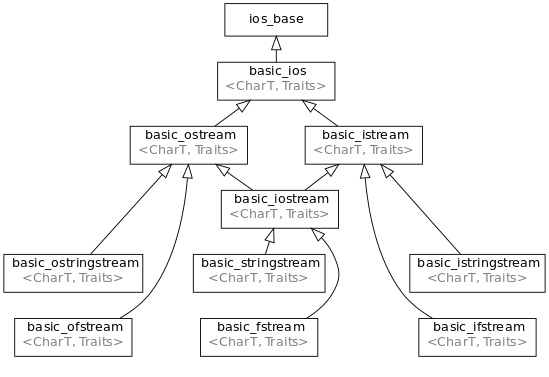
\includegraphics[width=.8\textwidth]{../images/generalized_parts/09_inheritance_diagram_of_io_library.png}
    \caption{C++流输入/输出库中的继承关系}
\end{figure}
我们曾经用 \lstinline@std::cout.setf(std::ios_base::boolalpha)@ 来改变 \lstinline@std::cout@ 对 \lstinline@bool@ 数据的输出方式,这里的 \lstinline@setf@ 和 \lstinline@fmtflags@ 其实都是定义在 \lstinline@std::ios_base@ 类中的。\lstinline@std::ostream@ 间接继承了 \lstinline@std::ios_base@ 类,所以它可以把 \lstinline@std::ios_base::setf@ 当作自己的成员函数来调用。\par
我们也曾用过 \lstinline@std::cin.clear()@ 这样的写法,这里的 \lstinline@clear@ 是定义在 \lstinline@std::basic_ios<CharT,Traits>@ 类中的一个成员函数。\lstinline@std::istream@ 类继承了 \lstinline@std::basic_ios<ChatT,Traits>@,所以它也能调用这个成员函数。\par
敏锐的读者可能发现了,图9.6中的 \lstinline@std::basic_iostream@ 类同时继承了 \lstinline@std::basic_ostream@ 和 \lstinline@std::basic_istream@ 类。这种操作叫作多重继承,我们会在第十章中讲解有关问题。\par
